\documentclass[
%draft%     uncomment to activate draft mode (see preamble/proofs)
]{article}   

% preamble -- do not rearrange order of \includes
%\include{classoptions}
%\include{pagesize}
%\include{packages}
%\include{encoding}         
%\include{fonts}
%\include{ToC}
%\include{contributor}
%\include{copyright}
%\include{bibtex}
%\include{environments}
%\include{sectionoptions}
%\include{headerfooter}
%\include{footnoteformat}
%\include{codesnipets}
%\include{proofs}
\usepackage{algorithm}% http://ctan.org/pkg/algorithms
\usepackage{algpseudocode}% http://ctan.org/pkg/algorithmicx
\usepackage{tikz}
\usepackage{graphicx}
\usepackage[export]{adjustbox}
\usepackage{caption}
\usepackage{amssymb}
\usepackage{float}
\usepackage{subfig}
\usepackage{placeins}
\usepackage{listings}
\lstset{
  basicstyle=\ttfamily,
  mathescape
}
%\usepackage{minted}
\usetikzlibrary{shapes}
\usetikzlibrary {positioning}
\usetikzlibrary{chains}
\usetikzlibrary{fit}
\usetikzlibrary{chains,shadows.blur}
\usepackage{geometry}
\usepackage{array}
\usepackage{hyperref}
\usepackage{indentfirst}
\hypersetup{
    colorlinks=true,
    linkcolor=magenta,
    filecolor=cyan,      
    urlcolor=blue,
}
\graphicspath{ {./images/} }


\usepackage{listings}
\usepackage{xcolor}

\definecolor{codegreen}{rgb}{0,0.6,0}
\definecolor{codegray}{rgb}{0.5,0.5,0.5}
\definecolor{codepurple}{rgb}{0.58,0,0.82}
\definecolor{backcolour}{rgb}{0.95,0.95,0.92}

\lstdefinestyle{mystyle}{
    % backgroundcolor=\color{backcolour},   
    commentstyle=\color{codegreen},
    keywordstyle=\color{magenta},
    numberstyle=\tiny\color{codegray},
    stringstyle=\color{codepurple},
    basicstyle=\ttfamily\footnotesize,
    breakatwhitespace=false,         
    breaklines=true,                 
    captionpos=b,                    
    keepspaces=true,                 
    numbers=left,                    
    numbersep=5pt,                  
    showspaces=false,                
    showstringspaces=false,
    showtabs=false,                  
    tabsize=2
}

\lstset{style=mystyle}


% define issue details
\title{Compiler Optimization Notes}
\newcommand\thejournalsubtitle{Notes compiled for the Compiler Optimization Course}
\newcommand\thevolume{}
\newcommand\theseason{May}
\newcommand\theyear{2022}
\newcommand\theissue{\thejournal \ \thevolume \ (\theyear)} 
\newcommand\generaleditor{}
\newcommand\associateeditor{}
\sloppy
\newcommand\thewebsite{https://github.com/liusy58/CompilerNotes}

\begin{document}
\sloppy                         % preferences more space between words over overrunning margins
\lefthyphenmin=3                % suppresses hyphenation after only 1 or 2 characters
                                % NB: You will need to repeat \lefthyphenmin in the text if you use \selectlanguage
%\include{editorialboard}
%\include{titlepage}
%\include{colofon}
\pagenumbering{roman}           
%\tableofcontents  
\thispagestyle{empty}

\maketitle

% \include{essays/preface}
\pagenumbering{arabic}

\section{Local Optimizations}

Local Optimizations never goes away because this is always a piece of what happens even when we 
talk about even more sophiscated types of optimizations.

First we will talk about how to represent the code within a function or procedure, that's using 
something called a flow graph which is made of basic blocks.  Next we will contrast two different 
abstractions for doing local optimizations.




\subsection{Basic Blocks/Flow graphs} 


\subsubsection{Basic Blocks}

A basic block is a sequence of instructions(3-address statements). There are some requirements for basic 
block:

\begin{itemize}
    \item \textbf{Only the first instruction can be reached from outside the blcok.} The reason why this property 
    is useful is that within a basic block, we just march instruction by instruction through the block, 
    this simplies things at least within a basic block.
    \item \textbf{All the statements are executed consecutively if the first one is.}
    \item \textbf{The basic block must be maximal.} i.e., they cannot be made larger without violating conditions. 
\end{itemize}


\subsubsection{Flow graphs}
Flow graph is a graph representation of the procedure. In flow graph, basic blocks are the nodes, and the edge for \(  B_i 
\rightarrow B_j \) stands for a path from node \( B_i \) to node \( B_j \). So how will \(  B_i  \rightarrow B_j \) happen? 
There are two possibilities:

\begin{itemize}
    \item Either first instruction of \(B_j\) is the target of a goto at end of \(B_i\).
    \item \(B_j\) physically follows \(B_i\) which doesn't end in an unconditional goto.
\end{itemize}




% \begin{center}

% \begin{tikzpicture}[auto,
%     node distance = 12mm,
%     start chain = going below,
%     box/.style = {draw,rounded corners,blur shadow,fill=white,
%           on chain,align=center}]
%    \node[box] (b1)    {$x_1\leftarrow0$\\ $y_1\leftarrow0$};      
%    \node[box] (b2)    {$x_2\leftarrow\phi(x_1,x_3)$\\
%    $y_2\leftarrow\phi(y_1,y_3)$\\
%    $(x_2<10)$?};      
%    \node[box] (b3)    {$y_3\leftarrow y_2+x_2$\\ $x_3\leftarrow x_2+1$};  
%    \node[box] (b4)    {print($y_2$)};     
%    \begin{scope}[rounded corners,-latex]
%     \path (b2.-40) edge[bend left=50] (b4.40)
%     (b1) edge (b2) (b2) edge (b3);
%     \draw (b3.230) -- ++(0,-0.3) -| ([xshift=-5mm]b2.west) |-
%     ([yshift=3mm]b2.130) -- (b2.130);
%    \end{scope}
%   \end{tikzpicture}

% \end{center}




\subsubsection{Partitioning into Basic Blocks}

\begin{itemize}
\item Identify the leader of each basic block 
    \begin{itemize}
        \item First instruction
        \item Any target of a jump
        \item Any instruction immediately following a jump
    \end{itemize}

\item Basic block starts at leader and ends at instruction immediately before a leader(or the last instruction).    
\end{itemize}

An example of flow graph is shown below:

\begin{figure}[h]
    \centering
    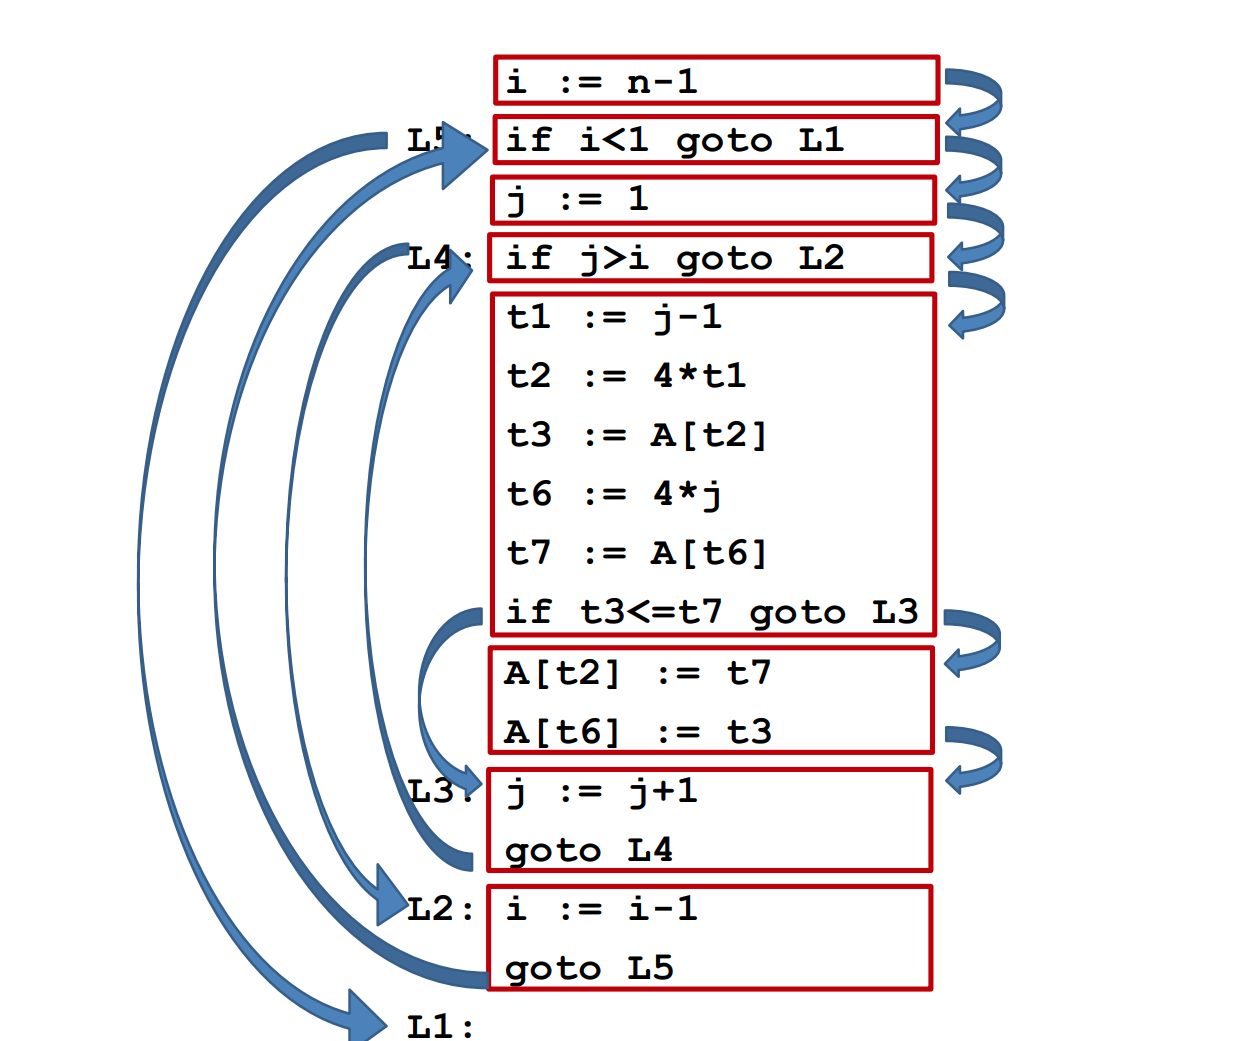
\includegraphics[width=0.5\textwidth]{flowgraph.png}
    \caption{Example of a flow graph}
\end{figure}

\subsubsection{Reachability of Basic Blocks}

There is one thing interesting need to mention here. So the source code is below:

\begin{lstlisting}[language=C, caption=An example]
if x { 
    ...
    return;
} else {
    ...
}


\end{lstlisting}


The corresponding flow graph is shown in \ref{fig:fgex}:

\begin{figure}[h]
    \centering
    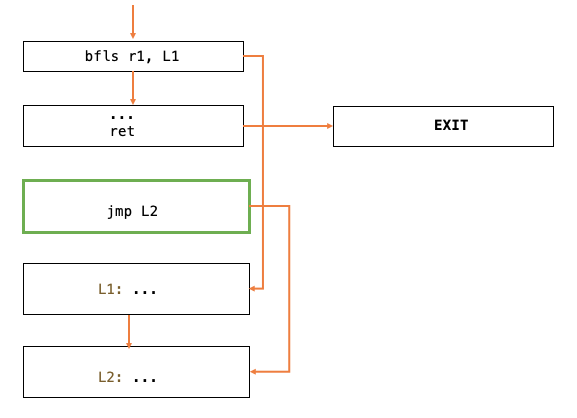
\includegraphics[width=0.5\textwidth]{fgex.png}
    \caption{Example of a flow graph}
    \label{fig:fgex}
\end{figure}


We can see that the box in green is unreachable from the entry. So why is that interesting? Typically, after compiers 
construct the control flow graph, they will go through and remove any unreachable nodes. Just do depth first traversal of the graph
from the entry node and mark all those visited nodes. So unmarked nodes will be deleted. This will help the compiler get a better optimization
result.


So why do these unreachable nodes appear? The anwser is it is not the job of the front-end of the compiler to clean up the unreachable nodes. 



\subsection{Local optimizations}

Local optimizations are those occur \textbf{within the basic blocks}. 


\subsubsection{common subexpression elimination}

There're some types of local optimizations. 
One is called \textbf{common subexpression elimination}. Subexpressions are some arithmetic expressions that occur on the
 right hand of the instructions. Common subexpressions are subexpression that occur many times where the operands have not 
 changed.
 
\begin{lstlisting}[language=C, caption=Subexpression example,label=lst:subexp]
a = b + c;
d = b + c;
\end{lstlisting}

In the example \ref{lst:subexp}, \texttt{b + c} is so called coomon subexpression, we could replace the instruction containing 
common subexpression with an assign expression. 


\begin{lstlisting}[language=C, caption=code snippet applied common subexpression elimination to \ref{lst:subexp},label=lst:transsubexpr]
    a = b + c;
    d = a
\end{lstlisting}

You may wonder why this kind of redundancy can occure in code? Are we programmers stupid to do so? In fact, 
the redundancy most comes from the stage when compilers  turn your source code. For example, when you use arrays,
you need to do some arithmetic to generate the address of the array element you are accessing. So every time you referece the same
array element, compiler will calculate the same address again. Similarly, if you access offsets within fields. Last example is 
access to parameters in the stack. 


\subsection{Abtraction 1:DAG}

DAG is the acronym for Directed Acyclic Graph. The Directed Acyclic Graph (DAG) is used to represent the 
structure of basic blocks, to visualize the flow of values between basic blocks, and to provide 
optimization techniques in the basic block. DAG is an efficient method for identifying common 
sub-expressions.\footnote{copied from \url{https://wildpartyofficial.com/what-is-dag-in-compiler-construction}}



The parse tree and DAG of the expression \(a + a*(b+c) + (b+c) *d \) is shown in \ref{fig:DAG}.


\begin{figure}[h]
    \centering
    \includegraphics[width=0.5\textwidth]{DAG.png}
    \caption{Example of a DAG}
    \label{fig:DAG}
\end{figure}



In DAG, some of the computation are reused. So we can generate optimizaed code based on DAG.

The optmized code for the DAG\ref{fig:DAG} is: 

\begin{lstlisting}[language=C, caption=code ,label=lst:dag]
    t1 = b - c;
    t2 = a * t1;
    t3 = a + t2;
    t4 = t1 * d;
    t5 = t3 + t4;
\end{lstlisting}


\subsubsection{How well do DAGs hold up across statements?}

We have seen that DAGs can be useful in a long arithmetic expression. So how well do DAGs
perform in sequence of instructions?

\begin{lstlisting}[language=C, caption=code ,label=lst:dagexpr2]
    a = b + c;
    b = a - d;
    c = b + c;
    d = a - d;
\end{lstlisting}


The corresponding DAG is shown in \ref{fig:DAG2}.
\begin{figure}[h]
    \centering
    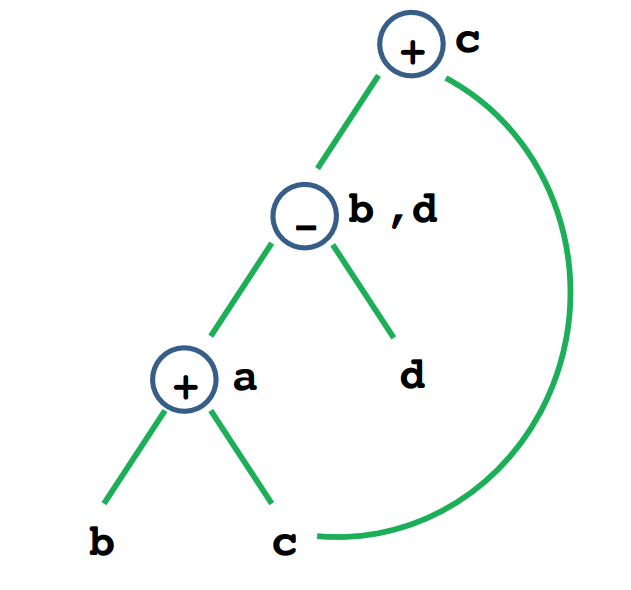
\includegraphics[width=0.5\textwidth]{dag2.png}
    \caption{Example of a DAG}
    \label{fig:DAG2}
\end{figure}

Based on the DAG\ref{fig:DAG2}, one optimizaed code is \ref{lst:dagexprop2}


\begin{lstlisting}[language=C, caption=code ,label=lst:dagexprop2]
a = b+c;
d = a-d;
c = d+c;
\end{lstlisting}

\ref{lst:dagexprop2} is not correct. B need to be overwritten but not yet. So if using DAGs, you need to be 
very careful. 

DAGs make sense if you just have one long expression, but once you have sequence of instructions overwriting variables
, DAGs are less appealing because this abstraction doesn't really include the concept of time.




\subsection{Abtraction 2:Value numbering} 

We have seen drawbacks of DAGs. One way to fix the problem is to attach variable name to latest value. Value numbering is 
such abstraction.

The idea behind value numbering is there is a mapping between variables(static) to values(dynamic). So common subexpression means same 
value number.

\subsubsection{Algorithm}


\begin{lstlisting}[language=python, caption=code ,label=lst:vna]
Data structure:
    VALUES = Table of
        expression /* [OP, valnum1, valnum2] */
        var /* name of variable currently holding expr */
For each instruction (dst = src1 OP src2) in execution order
    valnum1=var2value(src1); valnum2=var2value(src2)

    IF [OP, valnum1, valnum2] is in VALUES
        v = the index of expression
        Replace instruction with: dst = VALUES[v].var
    ELSE
        Add
            expression = [OP, valnum1, valnum2]
            var = tv
        to VALUES
        v = index of new entry; tv is new temporary for v
        Replace instruction with: tv = VALUES[valnum1].var OP VALUES[valnum2].var
                                dst = tv
    set_var2value (dst, v)  
\end{lstlisting}


\subsubsection{example}







\section{Introduction to Data Flow Analysis}

\subsection{Motivation for Dataflow Analysis}

Some optimizations\footnote{based on \url{https://pages.cs.wisc.edu/~horwitz/CS704-NOTES/2.DATAFLOW.html}} , however, require more "global" information. 
For example, consider the code \ref{lst:expr1}

\begin{lstlisting}[language=C,frame=single, caption=An ,label = lst:expr1]
    a = 1;
    b = 2;
    c = 3;
    if (...) x = a + 5;
    else x = b + 4;
    c = x + 1;
\end{lstlisting}


In this example, the initial assignment to \textit{c} (at line 3) is useless, and the expression 
\textit{x + 1} can be simplified to 7, but it is less obvious how a compiler can discover these facts 
since they cannot be discovered by looking only at one or two consecutive statements. 
A more global analysis is needed so that the compiler knows at each point in the program:
\begin{itemize}
\item    which variables are guaranteed to have constant values, and
\item    which variables will be used before being redefined.
\end{itemize}

To discover these kinds of properties, we use dataflow analysis. 



\subsubsection{What is Data Flow Analysis?}

Local Optimizations only consider optimizations within a node in CFG. 
Data flow analysis will take edges into account, which means composing 
effects of basic blocks to derive information at basic block boundaries.
Data-flow analysis is a technique for gathering information about the possible 
set of values calculated at various points in a computer program. A program's 
control-flow graph (CFG) is used to determine those parts of a program to which 
a particular value assigned to a variable might propagate. The information gathered 
is often used by compilers when optimizing a program. 


Typically, we will do local optimization for the first step to know what happens in a 
basic block, step 2 is to do data flow analysis. In he third step, we will go back and 
revisit the individual instructions inside of the blocks.


Data flow analysis is \textbf{flow-sensitive}, which means we take into account
 the effect of control flow. It is also a \textbf{intraprocedural analysis} which means
 the analysis is within a procedure. Data-flow analysis computes its solutions over the paths in
 a control-flow graph. The well-known, meet-over-all-paths
 formulation produces safe, precise solutions for general dataflow problems. All paths-whether feasible or infeasible,
 heavily or rarely executed-contribute equally to a solution. 

Here are some examples of intraprocedural optimizations:

\begin{itemize}
\item \textbf{constant propagation}. Constant propagation is a well-known global flow analysis 
problem. The goal of constant propagation is to discover values that are constant on all possible 
executions of a program and to propagate these constant values as far forward through the program 
as possible. Expressions whose operands are all constants can be evaluated at compile time and the 
results propagated further.

\item \textbf{common subexpression elimination}

\item \textbf{dead code elimination}. Actually, source code written by programmers doesn't contain
 a lot of dead code, dead code happens to occur partly because of how the front end translates code into 
 the IR. Doing optimizations will also turn code into dead.

\end{itemize}

% \subsection{Static    Program    vs.    Dynamic    Execution }

% Static program 




\subsubsection{Static Program vs. Dynamic Execution}


Program is statically infinite, but there can be infinite many dynamic execution paths. On one hand, analysis
 need to be precise, so we will take into account as much dynamic execution as possible. On the other hand, analysis
 need to do the analysis quickly. For a compromise, the analysis result is \textbf{conservative} and what it does id for each 
 point in the program, combines information of all the instances of the same program point.





\subsubsection{Data Flow Analysis Schema}
Before thinking about how to define a dataflow problem, note that there are two kinds of problems:
\begin{itemize}
    \item Forward problems (like constant propagation) where the information at a node n summarizes what can happen on paths from "enter" to n. So if we care about what happened in the past, it's a forward problem.
    \item Backward problems (like live-variable analysis), where the information at a node n summarizes what can happen on paths from n to "exit". So if we care about what will happen in the future, it's a backward problem.
\end{itemize}    

In what follows, we will assume that we're thinking about a forward problem unless otherwise specified.
 
Another way that many common dataflow problems can be categorized is as may problems or must problems. 
The solution to a "may" problem provides information about what may be true at each program point (e.g., 
for live-variables analysis, a variable is considered live after node n if its value may be used before 
being overwritten, while for constant propagation, the pair (x, v) holds before node n if x must have the value v at that point).

Now let's think about how to define a dataflow problem so that it's clear what the (best) solution should be. 
When we do dataflow analysis "by hand", we look at the CFG and think about:

\begin{itemize}
    \item What information holds at the start of the program.
    \item When a node n has more than one incoming edge in the CFG, how to combine the incoming 
    information (i.e., given the information that holds after each predecessor of n, how to 
    combine that information to determine what holds before n).
    \item How the execution of each node changes the information.
\end{itemize}    

This intuition leads to the following definition. An instance of a dataflow problem includes:
\begin{itemize}
    \item a \(CFG\),
    \item a domain \(D\) of "dataflow facts",
    \item a dataflow fact "init" (the information true at the start of the program for forward problems, 
    or at the end of the program for backward problems),
    \item an operator \(\wedge\) (used to combine incoming information from multiple predecessors),
    \item for each CFG node n, a dataflow function \(f_n\) :\( D \rightarrow D\) (that defines the effect of 
    executing n).
\end{itemize} 

For constant propagation, an individual dataflow fact is a set of pairs of the form (var, val),
 so the domain of dataflow facts is the set of all such sets of pairs (the power set). 
 For live-variable analysis, it is the power set of the set of variables in the program.

For both constant propagation and live-variable analysis, the "init" fact is the empty set 
(no variable starts with a constant value, and no variables are live at the end of the program).



For constant propagation, the combining operation \(\wedge\) is set intersection. 
This is because if a node n has two predecessors, p1 and p2, then variable x has value v before 
node n iff it has value v after both p1 and p2. For live-variable analysis, 
\(\wedge\) is set union: if a node n has two successors, s1 and s2, then the value of x after n may be 
used before being overwritten iff that holds either before s1 or before s2. In general, 
for "may" dataflow problems, \(\wedge\) will be some union-like operator, while it will be an intersection-like 
operator for "must" problems.

For constant propagation, the dataflow function associated with a CFG node that does not assign 
to any variable (e.g., a predicate) is the identity function. For a node n that assigns to 
a variable x, there are two possibilities:

\begin{itemize}
\item 1. The right-hand side has a variable that is not constant. In this case, the function 
result is the same as its input except that if variable x was constant the before n, 
it is not constant after n.
\item 2. All right-hand-side variables have constant values. In this case, the right-hand side of 
the assignment is evaluated producing consant-value c, and the dataflow-function result is the 
same as its input except that it includes the pair (x, c) for variable x (and excludes the pair 
for x, if any, that was in the input).
\end{itemize}


For live-variable analysis, the dataflow function for each node n has the form: 
\(f_n(S) = Gen_n \cup (S - KILL_n)\), where \(KILL_n\) is the set of variables defined at node n, 
and \(GEN_n\) is the set of variables used at node n. In other words, for a node that does not 
assign to any variable, the variables that are live before n are those that are live after 
n plus those that are used at n; for a node that assigns to variable x, the variables that are 
live before n are those that are live after n except x, plus those that are used at n 
(including x if it is used at n as well as being defined there).

An equivalent way of formulating the dataflow functions for live-variable analysis is: 
\(f_n(S) = (S \cap NOT-KILL_n) \cup GEN_n\), where \(NOT-KILL_n\) is the set of variables not defined
 at node n. The advantage of this formulation is that it permits the dataflow facts to be 
 represented using bit vectors, and the dataflow functions to be implemented using simple 
 bit-vector operations (and or).

It turns out that a number of interesting dataflow problems have dataflow functions of this 
same form, where \(GEN_n\) and \(KILL_n\) are sets whose definition depends only on n, and the combining 
operator \(\wedge\) is either union or intersection. These problems are called GEN/KILL problems, 
or bit-vector problems.




\subsection{Reaching Definitions}

The Reaching Definitions Problem is a data-flow problem used to answer the
following questions: Which definitions of a variable \textit{X} reach a given use of \textit{X} in
an expression? Is \textit{X} used anywhere before it is defined? A definition\textit{d} reaches a point \textit{p} if there exists path 
from the point immediately following \textit{d} to \textit{p} such that \textit{d} is not killed(overwritten) along that path.



\subsubsection{Iterative   Algorithm}

Here is the iterative  algorithm.



\begin{algorithm}
    \caption{Reaching Defintions:Iterative Algorithm}\label{alg:reachingdefiterative}
    \hspace*{\algorithmicindent} \textbf{Input: control flow graph CFG = (N, E, Entry, Exit) } \\
   
    
    \begin{algorithmic}
   
    \State out[Entry] = $\emptyset$ \algorithmiccomment{Boundary condition}

    \For{\texttt{each basic block B other than Entry}}
        \State \texttt{out[B] = $\emptyset$} \algorithmiccomment{Initialization for iterative algorithm }
    \EndFor
    \While{Changes to any out[] occur}
        \For{\texttt{each basic block B other than Entry}}
        \State \texttt{$in[B] =  \cup (out[p])$, for all predecessors p of B}
        \State \texttt{$out[B] = f_B(in[B])$} \algorithmiccomment{$out[B]=gen[B]\cup (in[B]-kill[B]) $ }
        \EndFor

    \EndWhile
    \end{algorithmic}
\end{algorithm}




\subsubsection{ Worklist   Algorithm}

\begin{algorithm}
    \caption{Reaching Defintions:Worklist Algorithm}\label{alg:reachingdefiterative}
    \hspace*{\algorithmicindent} \textbf{Input: control flow graph CFG = (N, E, Entry, Exit) } \\
   
    
    \begin{algorithmic}
   
    \State out[Entry] = $\emptyset$ \algorithmiccomment{Boundary condition}
    \State \textcolor{blue}{ChangedNodes = N}   
    \For{\texttt{each basic block B other than Entry}}
        \State \texttt{out[B] = $\emptyset$} \algorithmiccomment{Initialization for iterative algorithm }
    \EndFor
    \While{ChangedNodes $\neq \emptyset$}
        \State \textcolor{blue}{Remove i from ChangedNodes}
        \State $in[B] =  \cup (out[p])$, for all predecessors p of B
        \State \textcolor{blue}{$oldout = out[i]$}
        \State $out[i] = f_i(in[i])$ \algorithmiccomment{$out[i]=gen[i]\cup (in[i]-kill[i]) $ }
        \If {\textcolor{blue}{oldout} $\neq out[i]$}

            \For{\texttt{all \textcolor{blue}{successors s of i}}}
                \State \textcolor{blue}{add s to ChangedNodes}
            \EndFor
        \EndIf

    \EndWhile
    \end{algorithmic}
\end{algorithm}



\subsubsection{Example}


\begin{figure}[!htb]
    \minipage{0.32\textwidth}
      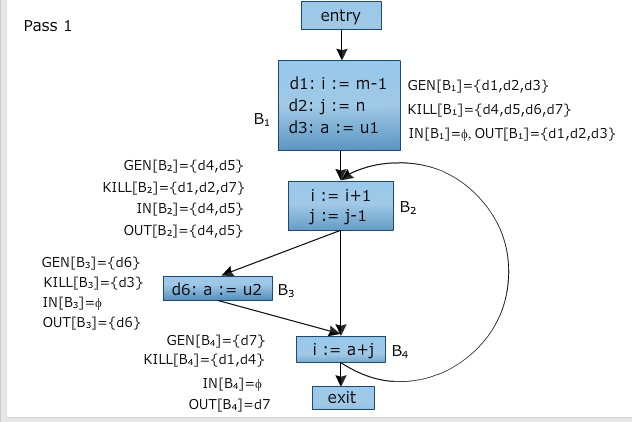
\includegraphics[width=\linewidth]{rdex1.jpg}
      \caption{Pass 1}\label{fig:awesome_image1}
    \endminipage\hfill
    \minipage{0.32\textwidth}
      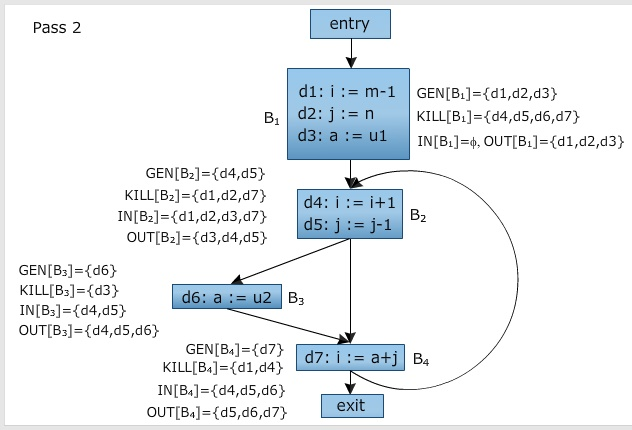
\includegraphics[width=\linewidth]{rdex2.jpg}
      \caption{Pass 2}\label{fig:awesome_image2}
    \endminipage\hfill
    \minipage{0.32\textwidth}%
      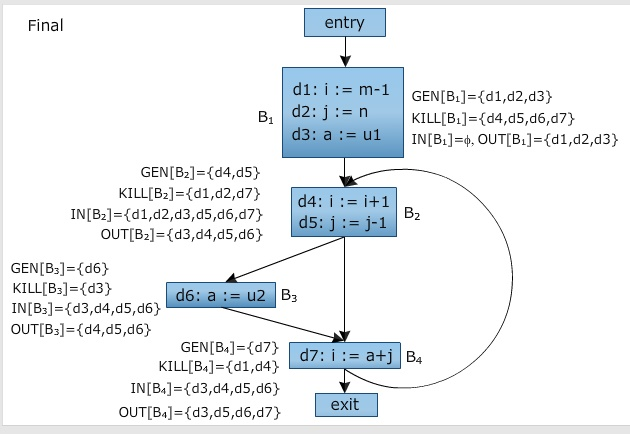
\includegraphics[width=\linewidth]{rdex3.jpg}
      \caption{Pass 3}\label{fig:awesome_image3}
    \endminipage
\end{figure}



\subsection{ Live    Variable    Analysis   }

In compilers, live variable analysis (or simply liveness analysis)
 is a classic data-flow analysis to calculate the variables that 
 are live at each point in the program. A variable is live at 
 some point if it holds a value that may be needed in the future, 
 or equivalently if its value may be read before the next time 
 the variable is written to. \footnote{based on Wikipedia}

\subsubsection{Motivation}


For dead code elimination.
\subsection{}



\end{document}
